\documentclass[]{jarticle}          % 一段組
%\documentclass[twocolumn]{jarticle} % 二段組

\textwidth 180mm
\textheight 255mm
\oddsidemargin -12mm
\topmargin -15mm
\columnsep 10mm

%\vspace{0.5cm} % 一段組の場合はコメントアウトした方が体裁がよいx
%] % 一段組の場合はコメントアウトする

\usepackage{styles/labheadings}
\usepackage[dvipdfmx]{graphicx,color}
\usepackage{amsmath,amssymb}
\usepackage{url}
% 追加
\usepackage[hang,small,bf]{caption}
\usepackage[subrefformat=parens]{subcaption}
\usepackage{float}
\captionsetup{compatibility=false}

\input{numerical_definition.tex}
% report.texと同じディレクトリにnumerical_definition.texを入れておけば上の書き方でもいいはずです

\usepackage[
  dvipdfm,
  bookmarks=true,
  bookmarksnumbered=true,
  colorlinks=true]{hyperref}
\AtBeginDvi{\special{pdf:tounicode EUC-UCS2}}

\pagestyle{labheadings}
\headerleft{全方位画像を用いたシーンの3次元モデルの作成とその活用}   % ヘッダの左側のタイトル
\headerright{2025年4月23日}  % ヘッダの右側のタイトル

\begin{document}

%\twocolumn % 一段組の場合はコメントアウトする

\vspace*{2ex}
\begin{center}
 {\Large \bf 3次元モデルの拡張}\\ % タイトル
 \vspace*{5mm}
 {\large M2 田川幸汰}% 発表者名
\end{center}

%\vspace{0.5cm} % 一段組の場合はコメントアウトした方が体裁がよいx
%] % 一段組の場合はコメントアウトする

%新しく作成したコマンド
% \newcommand{\reffig}[1]{\hyperref[#1]{図\ref{#1}}}
% \newcommand{\refeq}[1]{\hyperref[#1]{式(\ref{#1})}}
% \newcommand{\reftab}[1]{\hyperref[#1]{表\ref{#1}}}
% \newcommand{\refsec}[1]{\hyperref[#1]{\ref{#1}章}}
% \newcommand{\refsubsec}[1]{\hyperref[#1]{\ref{#1}節}}

% 数式
%\begin{equation}
%  数式記述  
%  \label{ラベル名}
%\end{equation}

% 図
% \begin{figure}[!ht]
%   \begin{center}
%     \includegraphics[scale=0.5]{figures/画像ファイル名}
%     \caption{キャプション名}
%     \label{ラベル名}
%   \end{center}
% \end{figure}

% リスト
% \begin{enumerate or itemize}
%   \item 
% \end{enumerate or itemize}

\section{概要}
より広範囲の環境を再現可能な3次元モデルを作成するため、モデルの構造を拡張した。
あわせて、拡張した範囲のテクスチャ情報を取得するために、全方位画像の撮影位置を従来より増やした。
各撮影位置に対応するカメラの外部パラメータの推定精度及び取得したテクスチャ、
テクスチャをカメラパラメータの推定結果をもとにモデルに割り当てた結果について示す。
  
\section{3次元モデルの拡張}
3次元モデルを図\ref{one}のように拡張した。
また、頂点はカメラのパラメータ推定を行う際の対応点として用いている。
\begin{figure}[H]
  \begin{center}
    \begin{tabular}{c}
      \includegraphics[width=0.9\textwidth]{figures/C5F_2dmap.png}
    \end{tabular}
  \end{center}
  \caption{3次元モデルの拡張}
  \label{one}
\end{figure}
青色が測定値、茶色が推定値となっているが、大きな誤差なく推定できていることがわかる。
\section{テクスチャの取得}
取得したテクスチャの一部を図\ref{two}に示す。
一部のテクスチャが、壁越しで取得してしまっている。ここについては
人力で取り除く方法が一番効率的だと考える。
また、画像の範囲に収まりきっていないテクスチャが選択されてしまうケースもみられる。
これについてはプログラムの不具合なので早急に直していきたい。
\begin{figure}[H]
  \begin{center}
    \begin{tabular}{cc}
      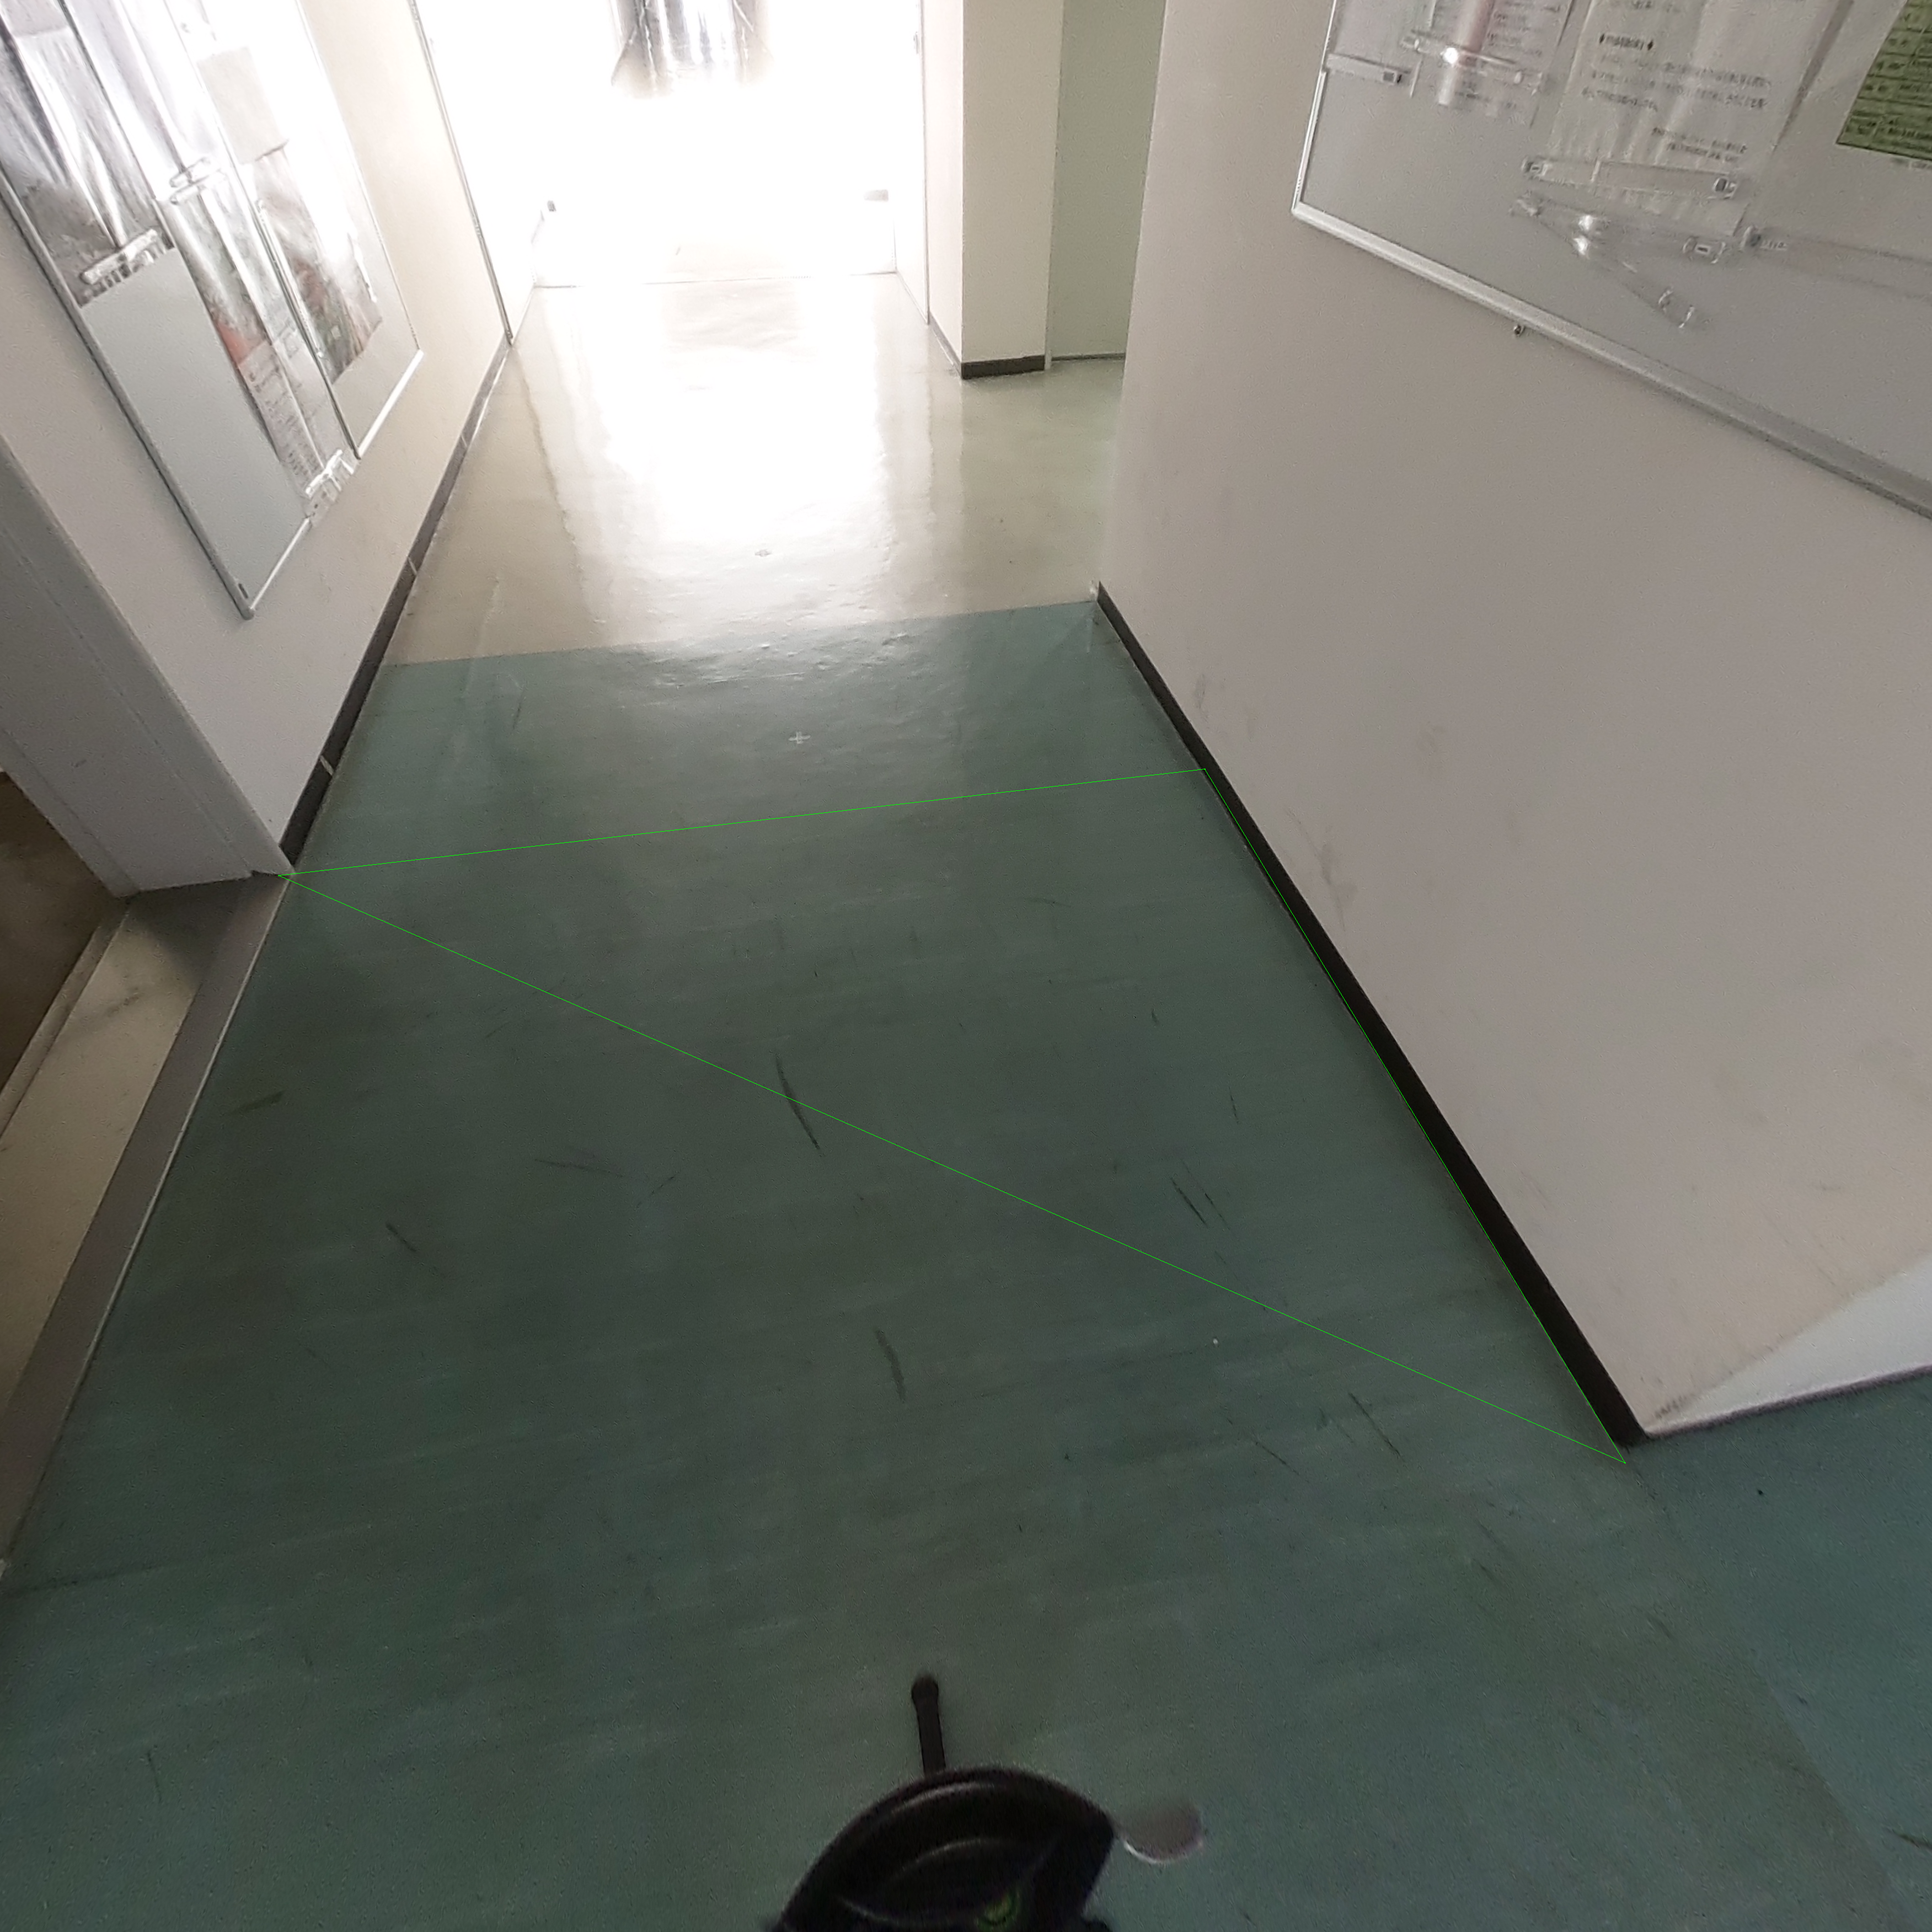
\includegraphics[width=0.4\textwidth]{figures/texture_1_7.png}&
      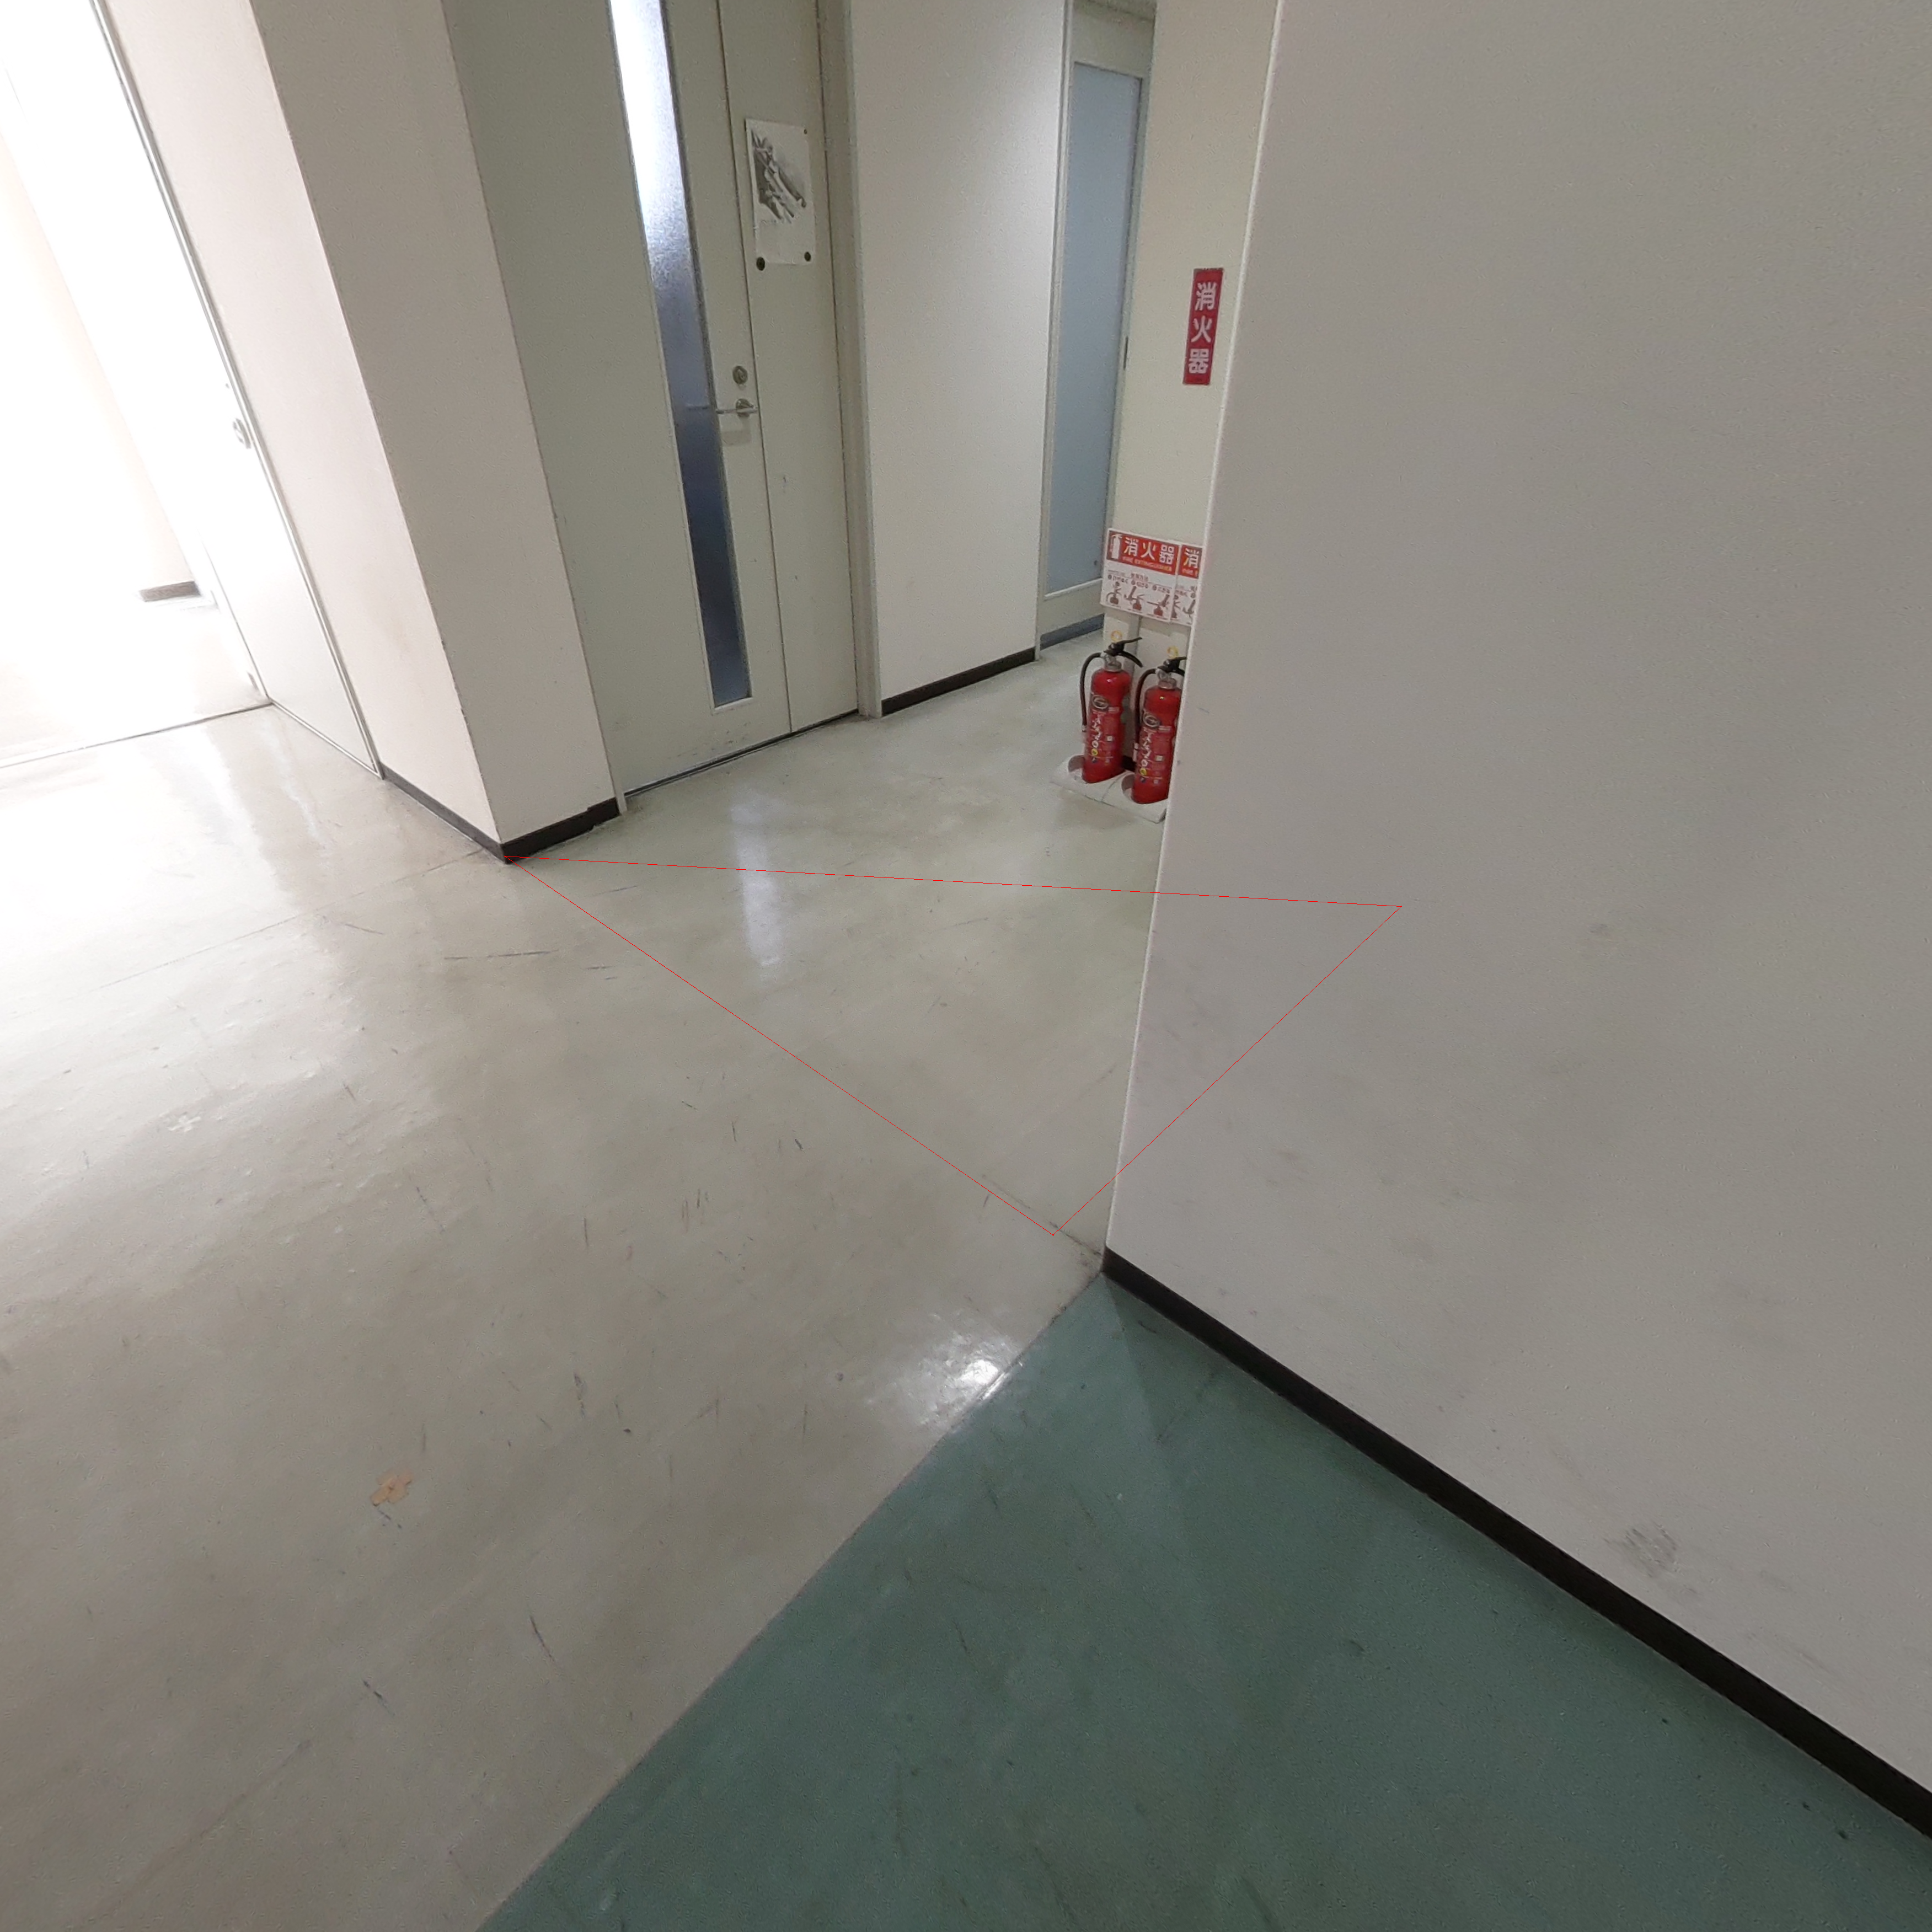
\includegraphics[width=0.4\textwidth]{figures/texture_2_12.png}\\
      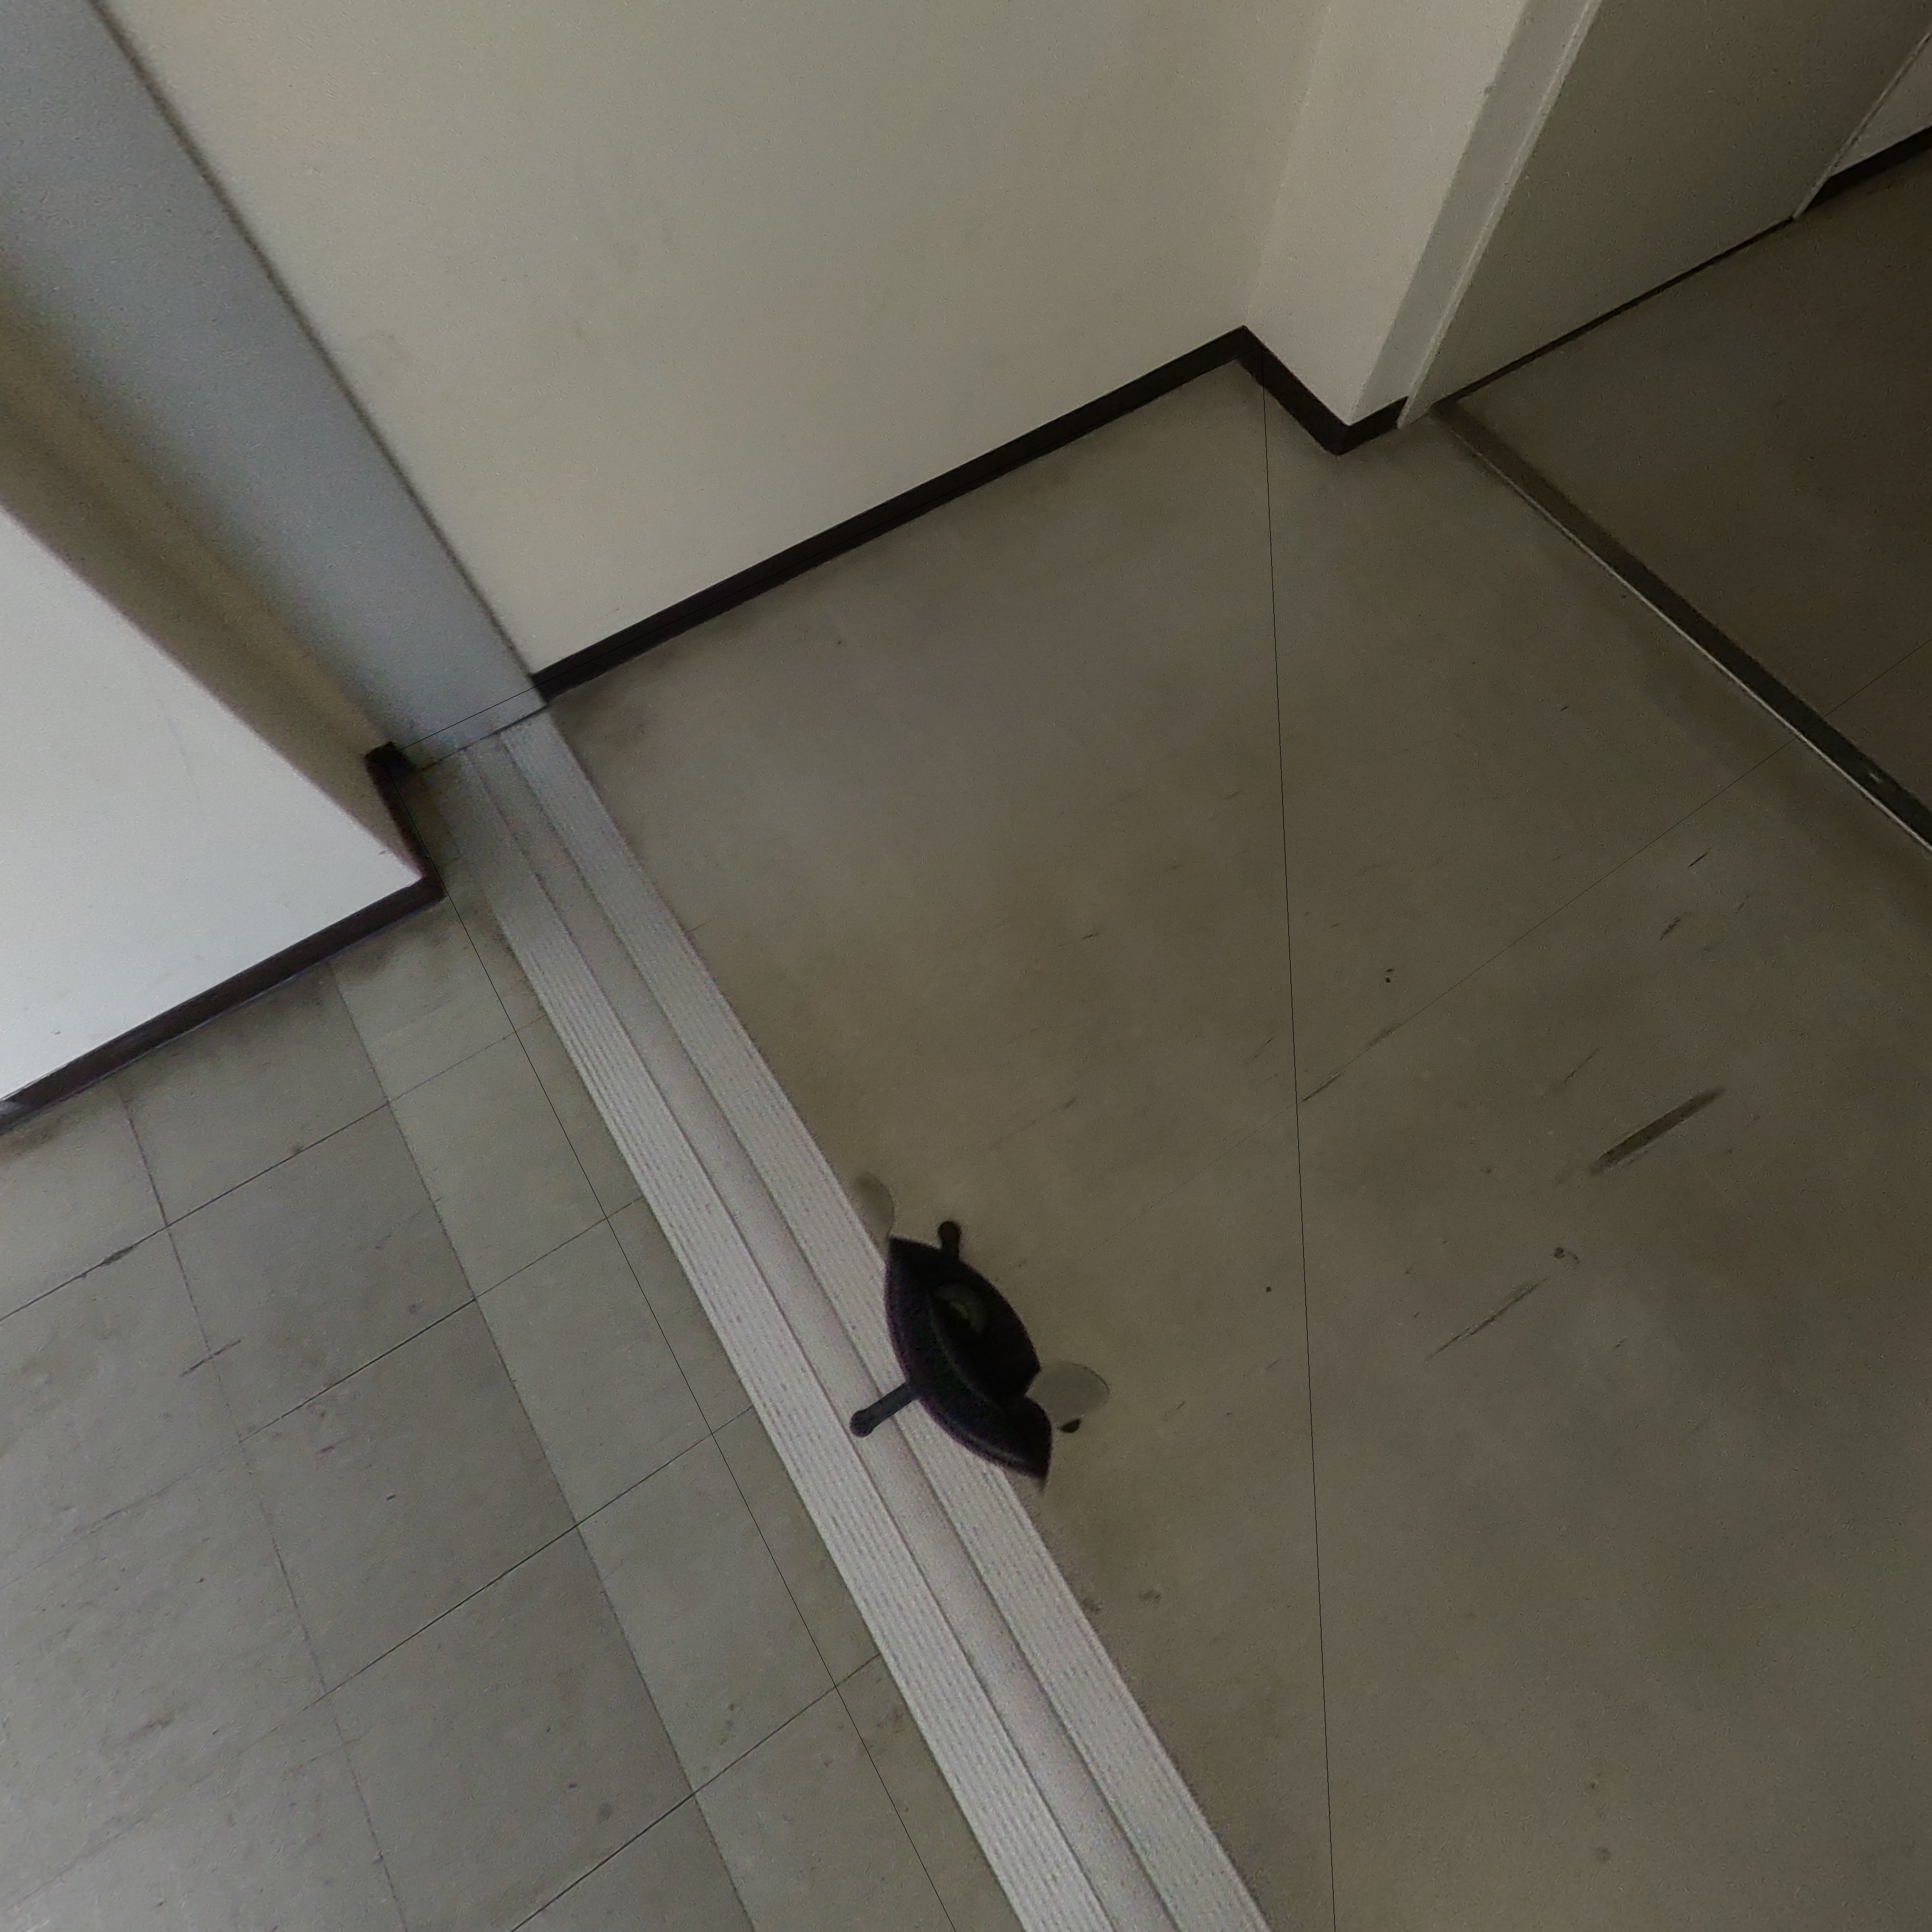
\includegraphics[width=0.4\textwidth]{figures/texture_5_19.png}&
      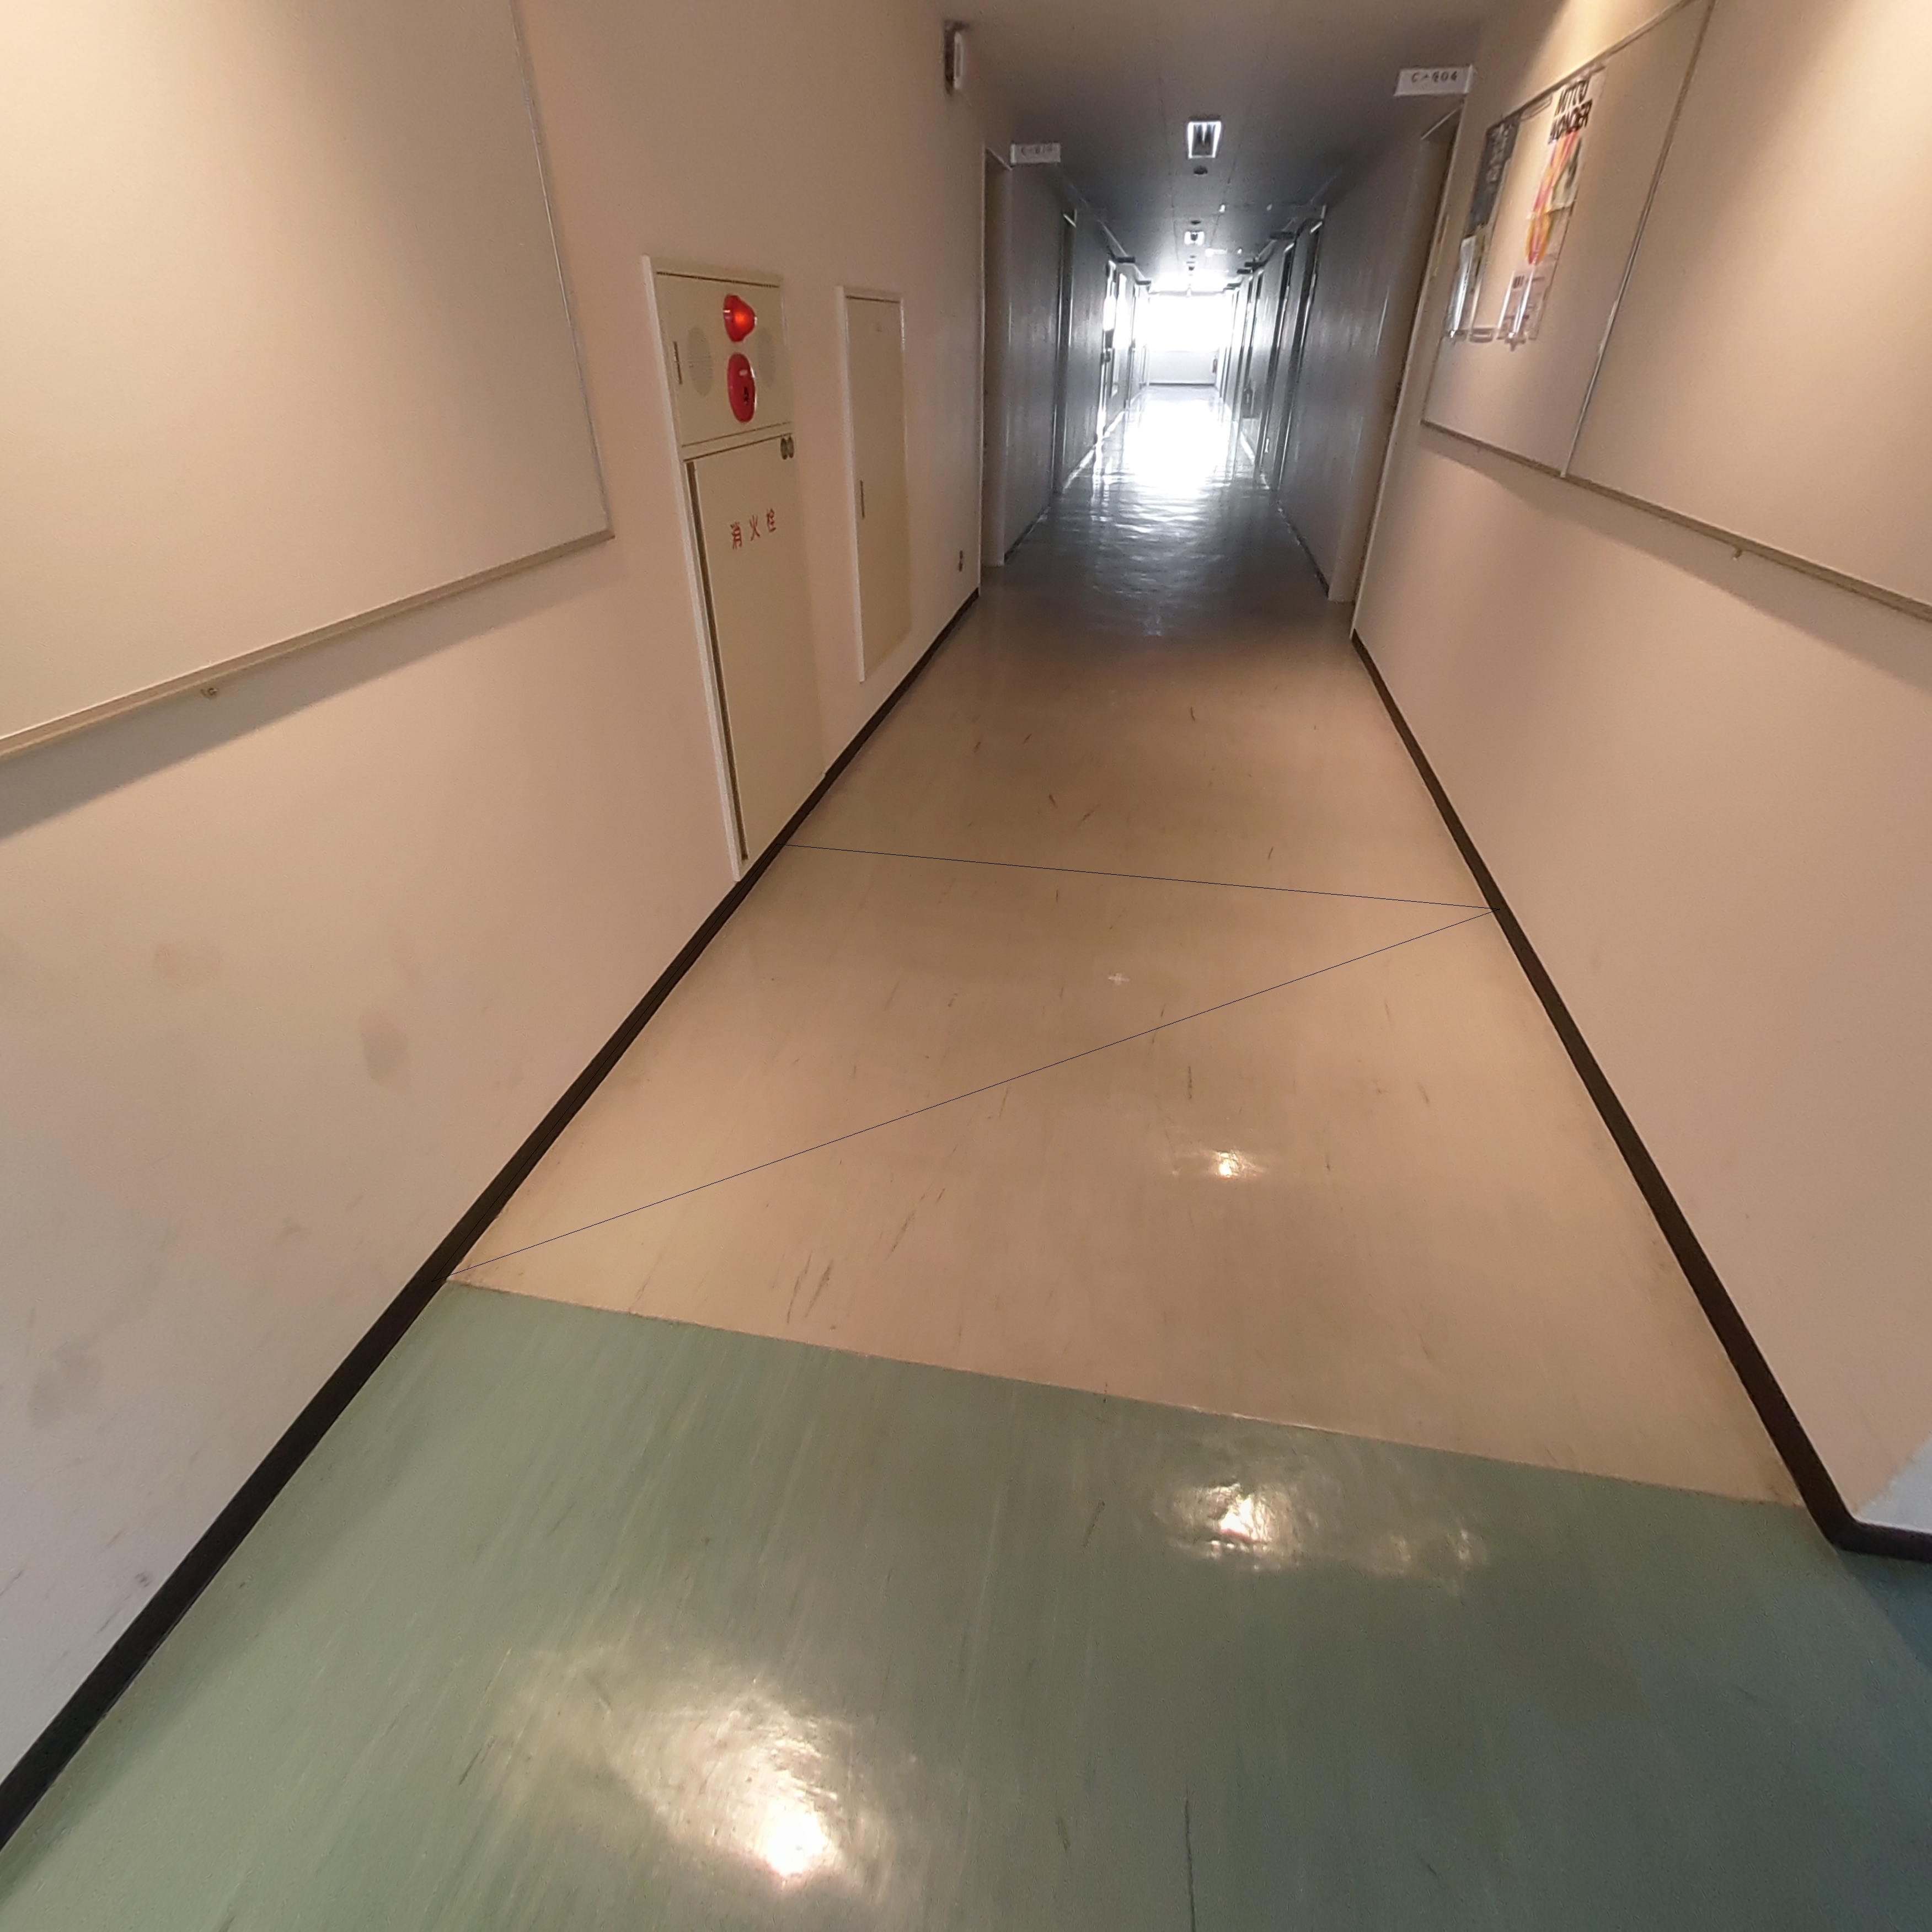
\includegraphics[width=0.4\textwidth]{figures/texture_8_47.png}\\
    \end{tabular}
  \end{center}
  \caption{テクスチャ画像}
  \label{two}
\end{figure}
\section{テクスチャの割り当て}
テクスチャを割り当てた3次元モデルを図\ref{three}に示す。
\begin{figure}[H]
  \begin{center}
    \begin{tabular}{c}
      \includegraphics[width=0.8\textwidth]{figures/3dmodel1.png}\\
      \includegraphics[width=0.8\textwidth]{figures/3dmodel2.png}\\
    \end{tabular}
  \end{center}
  \caption{3次元モデル}
  \label{three}
\end{figure}
床面の再現精度は現時点で十分ではなく、これはテクスチャ取得時の誤差や、
側面のように射影変換を行っていないことによるひずみが原因と考えられる。
本研究では床面を自己位置推定に用いていないため直接的な影響は少ないが、
モデル全体の再現性向上のためには改善が望ましい。

以前は、三角形メッシュを細かく分割することでひずみを軽減できたが、
大規模モデルでは作業負担が大きくなる。
今後はメッシュの自動分割により、再現精度と作業効率の両立を図りたい。

また、光による影も課題であり、
曇天時の再撮影や、画像間の輝度調整によって影響を軽減することを検討している。


\section{今後の計画}
今後の研究計画を以下に示す。
\begin{enumerate}
  \item 拡張した3次元モデルの側面部のテクスチャ割り当て
  \item 自己位置推定機能を応用した実用的なアプリケーションの開発
  \begin{itemize}
    \item 生成された3次元モデルと自己位置推定を組み合わせ、目的地までのルートを提示するナビゲーションシステムを構築
  \end{itemize}
\end{enumerate}
\end{document}
